% This text is proprietary.
% It's a part of presentation made by myself.
% It may not used commercial.
% The noncommercial use such as private and study is free
% Sep. 2005 
% Author: Sascha Frank 
% University Freiburg 
% www.informatik.uni-freiburg.de/~frank/



\pdfminorversion=5
\pdfobjcompresslevel=3 
\pdfcompresslevel=9

% Full presentation (with overlays, animated bullet items etc)
\documentclass[xcolor={x11names,svgnames,dvipsnames}]{beamer}

% Transparency mode (no overlays)
%\documentclass[xcolor={x11names,svgnames,dvipsnames},trans]{beamer}

% 4-up handout mode
%\documentclass[xcolor={x11names,svgnames,dvipsnames},handout]{beamer}

\usepackage{pgfpages}

\usepackage[british]{babel}
\usepackage{etex}

%% Glossy pretty look for the presentation and transparency (w/o overlays and animations) versions!
\mode<beamer|trans>{
	\useoutertheme[glossy]{wuerzburg}
	\useinnertheme[shadow,outline]{chamfered}
	\usecolortheme{shark}
}
\setbeamertemplate{navigation symbols}{}
\setbeamertemplate{frametitle continuation}[from second][(cont'd)]
\usefonttheme[stillsansseriftext,stillsansserifsmall]{serif}

%% Save up on ink for the 4-up handouts
\mode<handout>{
	\useoutertheme{wuerzburg}
	\useinnertheme[outline]{chamfered}
	\pgfpagesuselayout{4 on 1}[a4paper, landscape, border shrink=10mm]
	\pgfpageslogicalpageoptions{1}{border code=\pgfstroke}
	\pgfpageslogicalpageoptions{2}{border code=\pgfstroke}
	\pgfpageslogicalpageoptions{3}{border code=\pgfstroke}
	\pgfpageslogicalpageoptions{4}{border code=\pgfstroke}
}

\mode<presentation>{\AtBeginSection{%
		\begin{frame}
			\frametitle{Contents}
			\tableofcontents[currentsection]
		\end{frame}}}
		
		\usepackage{microtype}
		\usepackage[utf8]{inputenc}
		\usepackage[T1]{fontenc}
		\usepackage[osfss]{libertine}
		\usepackage[scaled=.77]{beramono}
		\usepackage{cmap}
		
		\usepackage{relsize,tabularx}
		\usepackage[T1,safe]{tipa}
		\usepackage{dtklogos,hologo,textcomp}
		\usepackage{multicol,booktabs}
		\usepackage{listings}
		\lstset{upquote,keepspaces=true,columns=spaceflexible,
			basicstyle=\ttfamily\scriptsize,%
			breaklines=true,breakindent=0pt,xleftmargin=0pt, xrightmargin=6pt,%
			language=[LaTeX]TeX, texcsstyle=*\bfseries\color{Maroon}, commentstyle=\sffamily\itshape\smaller\color{SeaGreen4},
			emphstyle=\bfseries\color{RoyalBlue3},escapechar={:},
			emphstyle={[2]{\bfseries\color{Sienna2}}},
			postbreak=\mbox{{\smaller\color{gray}$\hookrightarrow$}}
		}
		
		\usepackage{tikz}
		\usetikzlibrary{shapes,arrows,positioning,matrix,chains,backgrounds,fit}
		
		\usepackage{multicol}
		\usepackage[version=3]{mhchem}
		\usepackage{chemfig}
		\usepackage{linguex,qtree}
		\let\fg\lingfg
		\usepackage{texshade}
		\usepackage[detect-all]{siunitx}
		\usepackage[siunitx]{circuitikz}
		\usepackage{bytefield}
		\usepackage{auto-pst-pdf}
		\usepackage{pstricks,pst-barcode}
		\usepackage{pgfplots}
		\usepackage{pgfgantt}
		\usepackage[skaknew]{chessboard,skak}
		\usepackage{cwpuzzle}
		\usepackage{gchords,guitar}
		\usepackage{spreadtab}
		\usepackage{ccicons}


\setlength\fboxsep{0pt}
\SetTracking{encoding=*}{-39}

\author[\textsc{Jian} Wang]{\textsc{Jian} Wang\\[1ex]%
{\small\url{wangjian790@gmail.com}\\[-.5ex]\url{}}\\
{\small{Financial math Ph.D Candidate}}\\
{\small{Florida State University}}\\
[0.8ex]\copyright\copyright\copyright\copyright} %\ccbyncsa}

\title{High frequency data trading}
%\titlegraphic{\ccbyncsa}
\date[\textsc{HFC} 2015]{High Frequency data Conference data Conference 2015 }%

% Include QR code of slides URL for presentation-mode only -- so that audience
%  can snap it and download it on the spot
\mode<beamer>{\titlegraphic{\begin{pspicture}\psbarcode[scalex=.75,scaley=.75]{http://liantze.penguinattack.org/latextypesetting.html\#mosc11-slides}{eclevel=L}{qrcode}\end{pspicture}}}

\hypersetup{%
pdfauthor={Jian Wang}, %% the "author" field from above includes garbage code...
pdfkeywords={HFC,Machine Learning,general}
}
\begin{document}
\begin{frame}
\maketitle
\end{frame}

%\title{Simple Beamer Class}   
%\author{Sascha Frank} 
%\date{\today} 

\frame{\frametitle{Table of contents}\tableofcontents} 


\section{High frequency trading}
\begin{frame}


\begin{block}{High frequency trading}
High frequency trading is a specialized case of algorithmic trading involving the frequent turnover of may positions of a security.
\end{block}

\begin{columns}
\column{2.3in}
\begin{block}{Positive impact }
\begin{itemize}
\item Increased liquidity
\item Narrowing spreads
\item Improve market efficiency
\item Increase fees for Exchanges  
\end{itemize}
\end{block}

\column{2.3in}
\begin{block}{Negative impact }
\begin{itemize}
\item Impact on the institutional investors.
\item Increase volatility 
\item Disadvantages to the small Investors
\end{itemize}
\end{block}
\end{columns}

\end{frame}

\begin{frame}

\textbf{\large{HFT Strategies:}}

\begin{columns}
\column{2.4in}
\begin{block}{Market Making}
\small{place bets on both sides of the trade by placing a limit order to
sell slightly above the current market price, or to buy slightly below the current
market price, thereby profiting from the difference between the two. }
\end{block}
\begin{block}{Liquidity Rebate Trading
 }
\small{look for large orders, fill a
part of that order, and then offer these shares back to the market by placing a limit order, which makes them eligible to collect the rebate fee for providing liquidity,with or without them making a capital gain.}
\end{block}
\column{2.5in}
\begin{block}{\alert{Statistical Arbitrage}}
\small{Firms and traders looking to make profits from market arbitrage essentially exploit
 the momentary inconsistencies in factors such as rates, prices, and other conditions
 between different exchanges or asset classes}
\end{block}
\begin{block}{Momentum Ignition }
\small{ ignition strategies involve initiating and canceling a number of trades and orders with a certain security in a particular direction, which may ignite a rapid market price movement.}
\end{block}
\end{columns}
\end{frame}


\section{DataSet}
\begin{frame}
\frametitle{Dataset}
The dataset is named stockdata which from huge package in R. It contained data that were
originally obtained from Yahoo! Finance. There are 1,258
observations representing 1,258 sequential trading days(form Jan 1 2003 to Jan 1 2008) and 452
variables, each of which was the day's closing price for a different
stock within the Standard \& Poor's 500.We also added two index into the data set, one is S\&P 500 and another is Nasdaq(so totally 454 variables).\\
Among all the stock data , we used Goldman Sachs stock return
series as our response variable and other stocks as the predictors to analyze the stock return series movement.
\begin{columns}
\column{2.3in}
\textbf{Company:}:
 \begin{figure}
     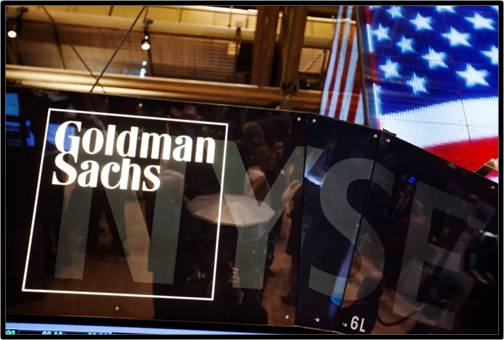
\includegraphics[width=0.6\textwidth, height=0.25\textheight]{gschart.jpg}
\end{figure}

\column{2.3in}

\textbf{Price:}:
\begin{figure}
     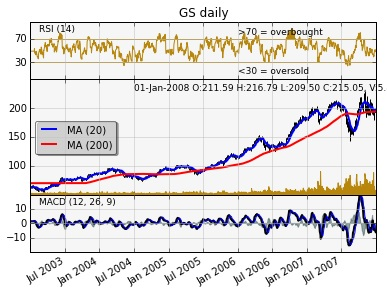
\includegraphics[width=0.6\textwidth, height=0.3\textheight]{gs_plot.jpg}
\end{figure}

\end{columns}
\end{frame}

\section{Methodology}

\begin{frame}
\frametitle{Methodology}
%
%\setbeamercovered{transparent}
%\begin{block}{Stock Return series}
%\begin{equation}
%R_t = ln( S_{t+1})-ln(S_t)
%\end{equation}
%Where $R_t$ is the stock return at trading day t and $S_t$ is the closing price of stock at trading day t.
%\end{block}
%\setbeamercovered{transparent}
\begin{block}{Logistic regression}
\begin{center}
$ln{\frac{F(x)}{1-F(x)}}=\beta_0+\sum_i\beta_ix_i$\\
\end{center}
\end{block}

\begin{block}{Ridge regression}
\begin{center}
$\hat{\beta}^{ridge}=argmin_{\beta}\{\sum_{i=1}^p{(y_i-\hat{y_i})^2}+{\color{red}\lambda \sum_{j=1}^p\beta_j^2}\}$
\\
\end{center}
\end{block}

\begin{block}{Lasso regression}
\begin{center}
$\hat{\beta}^{lasso}=argmin_{\beta}\{\sum_{i=1}^p{(y_i-\hat{y_i})^2}+{\color{red}\lambda\sum_{j=1}^p |\beta_j|}\}$\\
\end{center}
\end{block}

\end{frame}


\begin{frame}
\frametitle{Methodology}
Comparison of L1 and L2 Penalized Model \\
\begin{columns}
\column{2.3in}
	\begin{block}{Ridge regression}
$\hat{\beta}^{ridge}=argmin_{\beta}\{\sum_{i=1}^p{(y_i-\hat{y_i})^2}+{\color{red}\lambda \sum_{j=1}^p\beta_j^2}\}$

\end{block}
\textbf{Coefficients}:
 \begin{figure}
     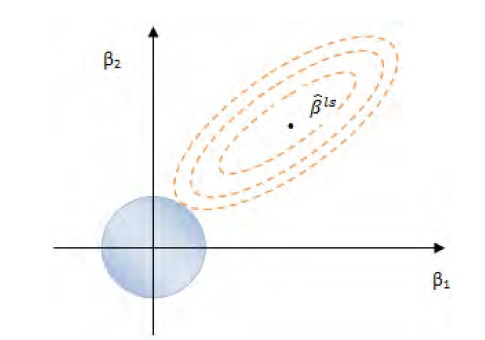
\includegraphics[width=0.9\textwidth, height=0.5\textheight]{ridge.jpg}

    \end{figure}

\column{2.3in}
\begin{block}{Lasso regression}

$\hat{\beta}^{lasso}=argmin_{\beta}\{\sum_{i=1}^p{(y_i-\hat{y_i})^2}+{\color{red}\lambda\sum_{j=1}^p |\beta_j|}\}$

\end{block}

\textbf{Coefficients}:
 \begin{figure}
     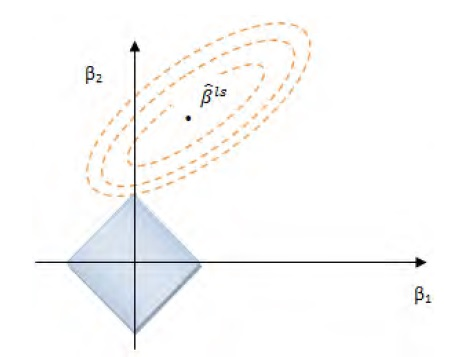
\includegraphics[width=0.9\textwidth, height=0.5\textheight]{lasso.jpg}
    \end{figure}
\end{columns}


\end{frame}

\begin{frame}
\frametitle{Methodology}
Comparison of L1 and L2 Penalized Model \\
\begin{columns}
\column{2.3in}
	\begin{block}{Ridge regression}
$\hat{\beta}^{ridge}=argmin_{\beta}\{\sum_{i=1}^p{(y_i-\hat{y_i})^2}+{\color{red}\lambda \sum_{j=1}^p\beta_j^2}\}$

\end{block}
\textbf{Path:}:
 \begin{figure}
     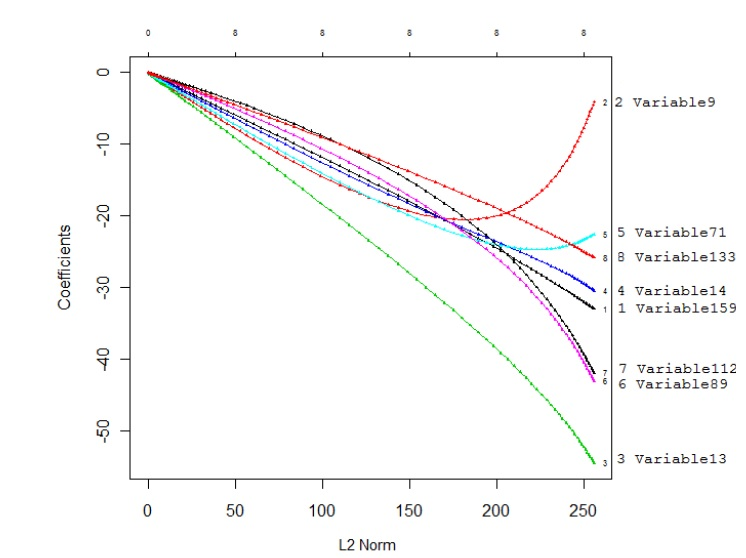
\includegraphics[width=0.9\textwidth, height=0.5\textheight]{ridge_p.jpg}

    \end{figure}

\column{2.3in}

\begin{block}{Lasso regression}

$\hat{\beta}^{lasso}=argmin_{\beta}\{\sum_{i=1}^p{(y_i-\hat{y_i})^2}+{\color{red}\lambda\sum_{j=1}^p |\beta_j|}\}$

\end{block}

\textbf{Path:}:
 \begin{figure}
     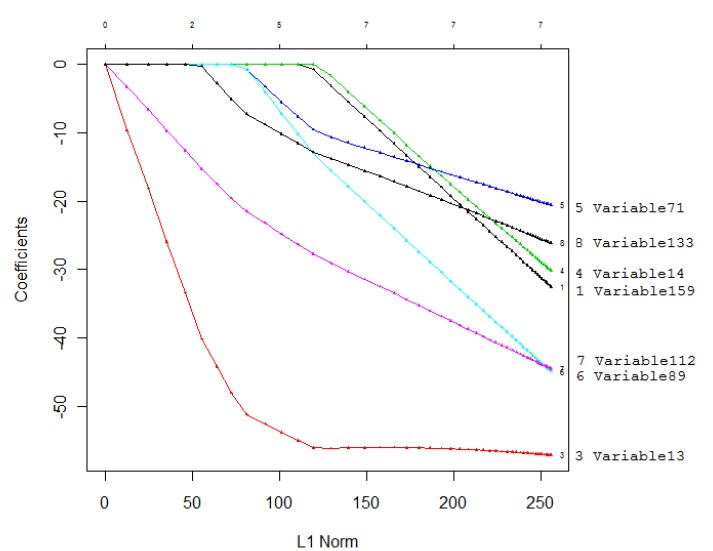
\includegraphics[width=0.9\textwidth, height=0.5\textheight]{lasso_p.jpg}

    \end{figure}
\end{columns}

\end{frame}

\begin{frame}
\frametitle{Methodology}
\begin{block}{Support vector machine}
{\small
• Introduced in COLT-92 by Boser, Guyon \& Vapnik. Became
rather popular since.\\
• Theoretically well motivated algorithm: developed from Statistical
Learning Theory (Vapnik \& Chervonenkis) since the 60s.\\
• Empirically good performance: successful applications in many
fields (bioinformatics, text, image recognition, . . . )\\
}
\end{block}

\begin{columns}<+->
\begin{column}{0.6\textwidth}
\small {
Try to maximize the margin:\\ 
$r=1/||w||,y_j=1,-1$\\
Primal form:\\
$\max\limits_{W,b}\ r= 1/||W||$\\
$s.t.(W^Tx_j+b)y_j>=1$\\
Dual form:\\
$\max\limits_{\alpha_1,...,\alpha_M}\ \sum\alpha_l-\frac{1}{2}\sum_{j=1}^{M}\sum_{k=1}^{M}\alpha_j\alpha_k y_j y_k<X_j,X_k>$\\
s.t.$\alpha_l\geq 0$, $\sum_{l=1}^{M}\alpha_ly_l=0$
}
\end{column}
\begin{column}{.4\textwidth}
     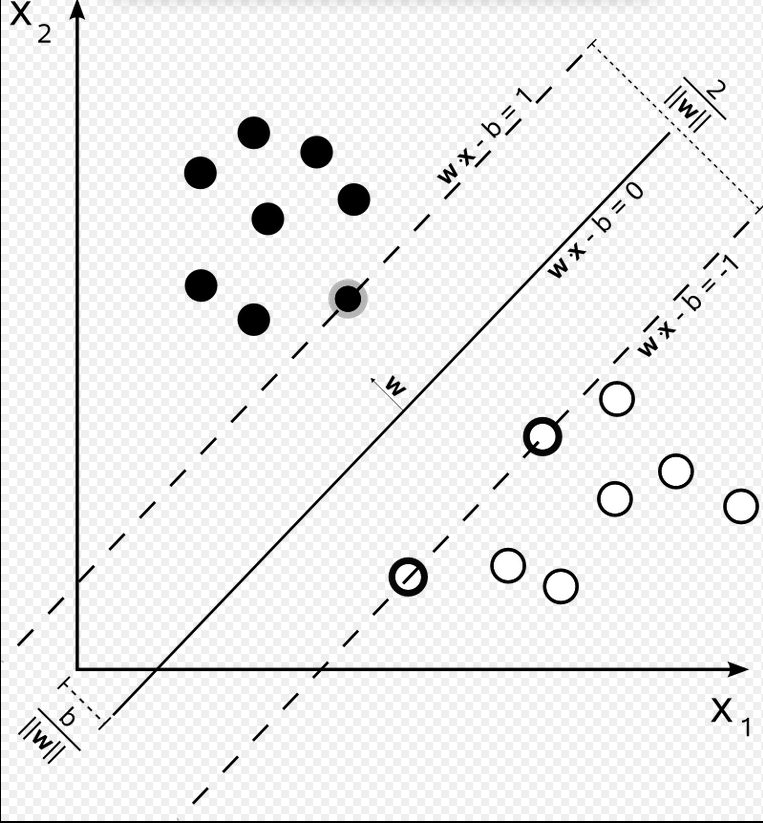
\includegraphics[width=0.8\textwidth, height=0.4\textheight]{svm.png}
\end{column}
\end{columns}
\end{frame}

\begin{frame}
\frametitle{Methodology}
\setbeamercovered{transparent}
\begin{block}{Kernel functions}
We can use the kernel function to calculate the inner product in high dimensional cases in its original feature spaces.
\end{block}
\begin{block}{Example:two dimension polinomial}
$k(x,z)=(x^Tz)^2$\\
$=(x_1^2,\sqrt{2}x_1x_2,x_2^2)^T(z_1^2,\sqrt{2}z_1z_2,z_2^2)$\\
$=\Phi(x)^T\Phi(z)$\\
\end{block}
\begin{block}{Kernel functions that we used}
\small{
\textbullet\ {Linear kernel:  $k(x,y)=x^Ty+c$}\\
\textbullet\ {Polynomial Kernel:  $k(x,y)=(\alpha x^Ty+c)^d$}\\
\textbullet\ {Radial basis function kernel(RBF):  $k(x,y)=exp(-\gamma||x-y||^2)$}
}
\end{block}

\end{frame}


\begin{frame}
\frametitle{Methodology}
  \setbeamercovered{transparent}
  \begin{block}{Glasso:}
    Suppose we have N multivariate normal observations of dimension p , with mean $\mu$ and covariacne $\Sigma$. Let $\Theta=\Sigma^{-1}$ and $S$ be the empirical covariance matrix, the problem is to maximize the log- likelihood \\
    \begin{center}
    $lnP(X|u,\Sigma)=-\frac{N}{2}ln|\Sigma|-\frac{1}{2}\sum(x_n-u)^T \Sigma^{-1}(x_n-u)$\\
    combined with the $L_1$ penalty\\
    $ln |\Theta|- tr(S\Theta))-\lambda||\Theta||_1$
  \end{center}
  \end{block}

  \begin{block}<2>{Algorithm}
  Many algorithms for this problem, The following might be the oldest and simple one by Meinshausen and Buhlmann(2006)
    \begin{itemize}
        \item  Estimate a sparse graphical model by fitting a lasso model to each variable, using others as predictors
        \item  Set $\Sigma_{ij}^{-1}$ to be non zero, if either the estimated coefficient of variable i on j, or the
        estimated coefficient of variable j on i, is non-zero
    \end{itemize}
  \end{block}
\end{frame}

\begin{frame}
\frametitle{Bayesian-Glasso model}
 For the high dimensional problem, it is not very easy to built the Bayesian network due to its exponentially increasing complexity. \\
 Our idea is to first use the Glasso model to conduct the model selection and then use Bayesian network structure learning process
 to define the network structure. \\
   \setbeamercovered{transparent}
   \begin{block}<2>{Algorithm}
    \begin{itemize}
        \item  Use Glasso algorithm to find the edges among variables
        \item  Use greedy search methods to change the direction only on those existed edges
        \item  Choose the direction which has the optimal BIC score
        \item  Finish when all the edges are reached or attain the maximum iteration numbers
    \end{itemize}
  \end{block}

\end{frame}




\begin{frame}
\frametitle{Methodology}
\setbeamercovered{transparent}
\begin{block}{Higher dimensional situations}
sometimes, in lower dimension we can not separate the data properly, so we need to project the data to the high dimensions\\
\end{block}
\begin{block}{Examples}
\begin{columns}
\column{2.3in}
\begin{figure}
     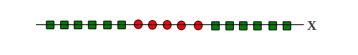
\includegraphics[width=0.5\textwidth, height=0.1\textheight]{1d.png}
\end{figure}
\begin{figure}
     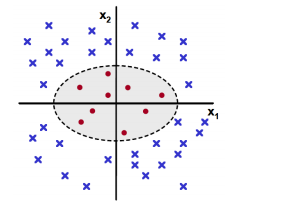
\includegraphics[width=0.5\textwidth, height=0.3\textheight]{2d.png}
\end{figure}

\column{2.3in}
\begin{figure}
     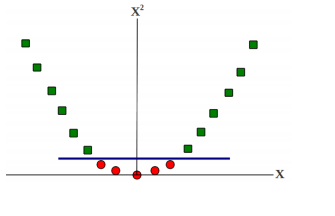
\includegraphics[width=0.5\textwidth, height=0.2\textheight]{1d_2.png}
\end{figure}
\begin{figure}
     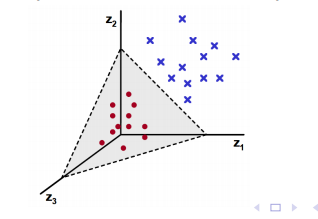
\includegraphics[width=0.5\textwidth, height=0.2\textheight]{2d_2.png}
\end{figure}
\end{columns}
\end{block}
\end{frame}


\begin{frame}
\frametitle{Methodology }
  \setbeamercovered{transparent}
  \begin{block}{Reference}
   \begin{itemize}
        \item  Tibshirani, R. (1996). "Regression shrinkage and selection via the lasso". Journal of the Royal Statistical Society, Series B 58 (1): 267–288. JSTOR 2346178
        \item Hoerl, A.E. and Kennard, R. (1970). Ridge regression: Biased
estimation for nonorthogonal problems. Technometrics, 12:
55-67
        \item Vapnik, V. (1995). "Support-vector networks". Machine Learning 20 (3): 273. doi:10.1007/BF00994018
    \end{itemize}
  \end{block}

  \begin{block}<2>{Packages}
    \begin{itemize}
        \item  R packages: glm, glmnet, e1071,bnlearn,huge
        \item  Python packages: sklearn (svm, ridge, lasso, logistic)
    \end{itemize}
  \end{block}

\end{frame}


\section{Numerical results}

\begin{frame}
\frametitle{Numerical results}
\begin{itemize}
        \item  Same day stock return series analysis:\\
        we use the same day stock return series to build the machine learning models. For the Bayesian network, we only use the R package. For the  logistic regression, ridge regression, lasso and svm, we used different languages(R and Python) and also compare the CPU time.
        To test the accuracy rate of model, we choose the first 1000 data as training data and the last remaining 257 data as testing. GS as response(discretized as 1 and -1) and the other 453 stocks as predictors.\\
        \item  Predict the stock data:\\
        we used the last one day, two day,... to last five day stock returns as the predictors and today's GS return series as response to see if our model can be used to predict the stockdata.\\
        Still use the first 1000 data as training and the remaining 252 data as testing. GS as the response and the other 2270 variables as predictors.\\
    \end{itemize}

\end{frame}

\begin{frame}
\frametitle{Numerical results}
\begin{block}{Bayesian network}
\begin{table}[h!]\small
  \caption{10 companies}
\begin{center}
    \begin{tabular}{| c | c| c | }
    \hline
    Stock code& Industry & Company name\\
    \hline
GS&Financials&Goldman Sachs Group\\
JPM&Financials&JPMorgan Chase \& Co.\\
MSFT&Information Technology&Microsoft Corp.\\
IBM&Information Technology&International Bus. Machines\\
T&Telecommunications Services&AT\&T Inc\\
VZ&Telecommunications Services&Verizon Communications\\
WMT&Consumer Staples&Wal-Mart Stores\\
KO&Consumer Staples&Coca Cola Co.\\
AMZN&Consumer Discretionary&Amazon.com Inc\\
BBY&Consumer Discretionary&Best Buy Co. Inc.\\

\hline
\end{tabular}
\end{center}
\end{table}
\end{block}

\end{frame}
\begin{frame}
\frametitle{Numerical results}
\setbeamercovered{transparent}

\begin{block}{Results for simple cases}
\begin{columns}
\column{1.5in}
\begin{figure}
     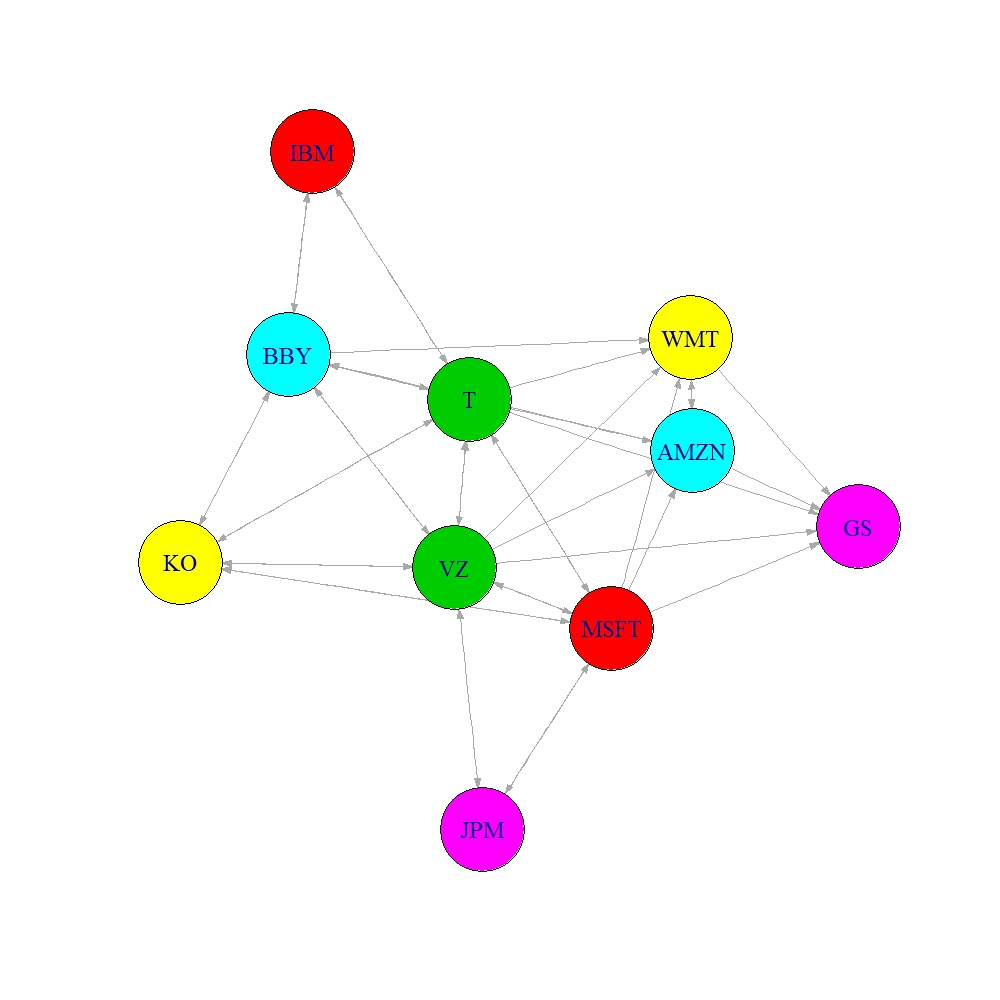
\includegraphics[width=1\textwidth, height=0.5\textheight]{10stocks.jpeg}
\end{figure}

\column{1.5in}
\begin{figure}
     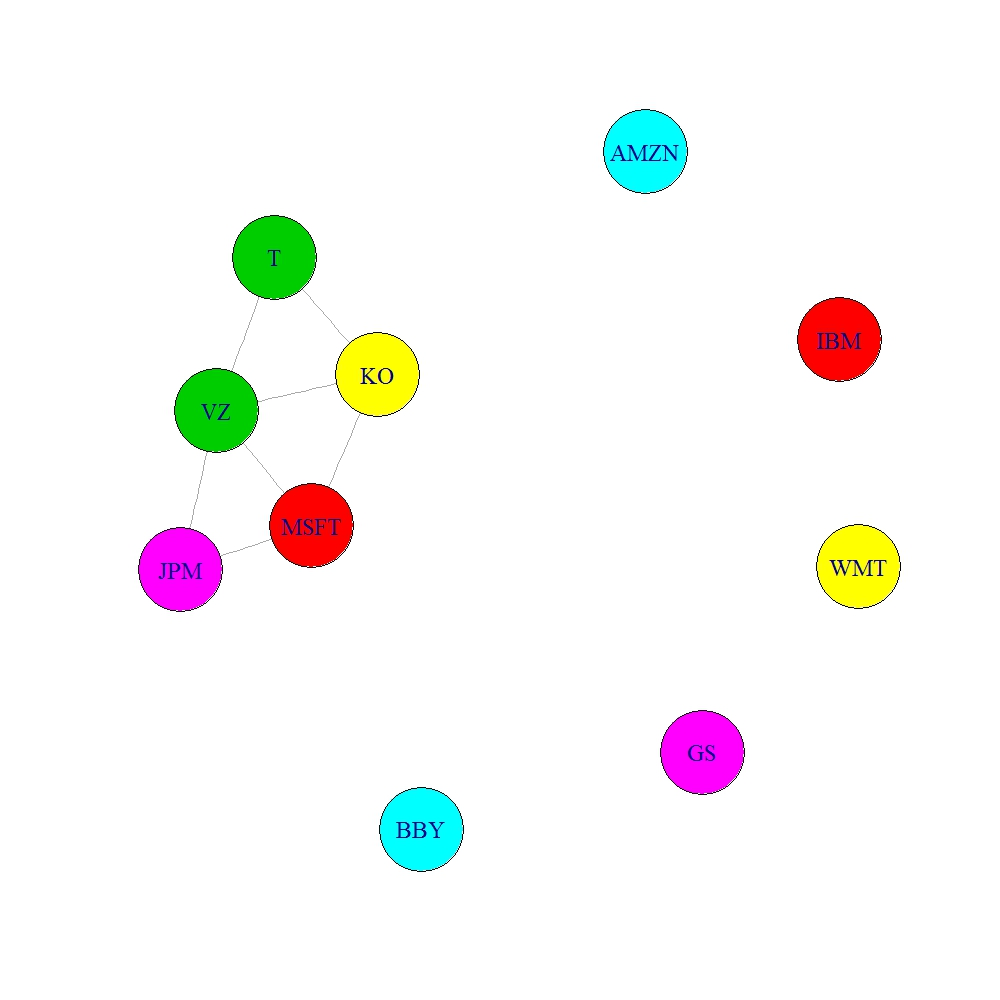
\includegraphics[width=1\textwidth, height=0.5\textheight]{10stocks_huge.jpeg}
\end{figure}
\column{1.5in}
\begin{figure}
     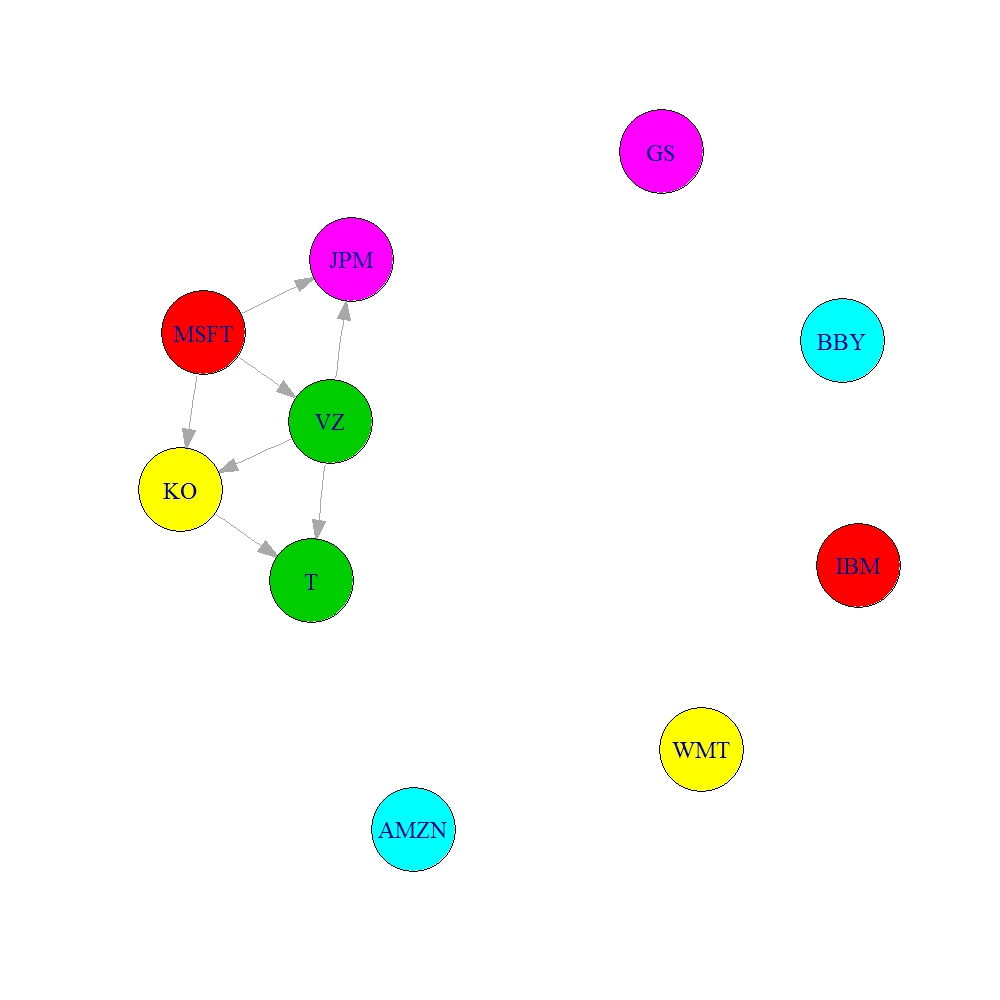
\includegraphics[width=1\textwidth, height=0.5\textheight]{10stocks_bn_glasso.jpeg}
\end{figure}
\end{columns}
\end{block}
\end{frame}

\begin{frame}
\frametitle{Numerical results}
\setbeamercovered{transparent}
\begin{block}{Results for total stocks}
     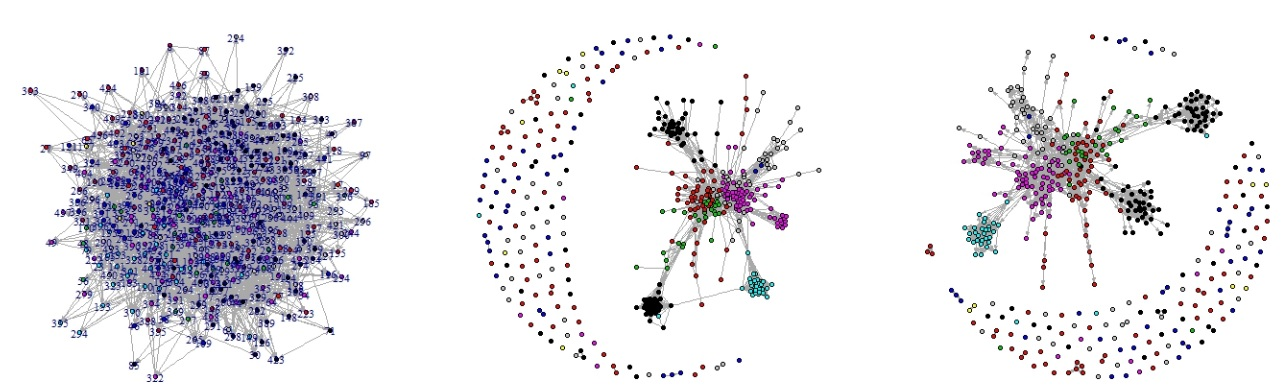
\includegraphics[width=0.9\textwidth, height=0.4\textheight]{stock.jpg}
\end{block}
\end{frame}

\begin{frame}
\frametitle{Numerical results}
\begin{columns}
\column{2.3in}
	\begin{block}{CPU Time for R}
We changed the number of samples from 50 to 800, doubled each time to test the running time for the different machine learning methods:\\
\begin{figure}
     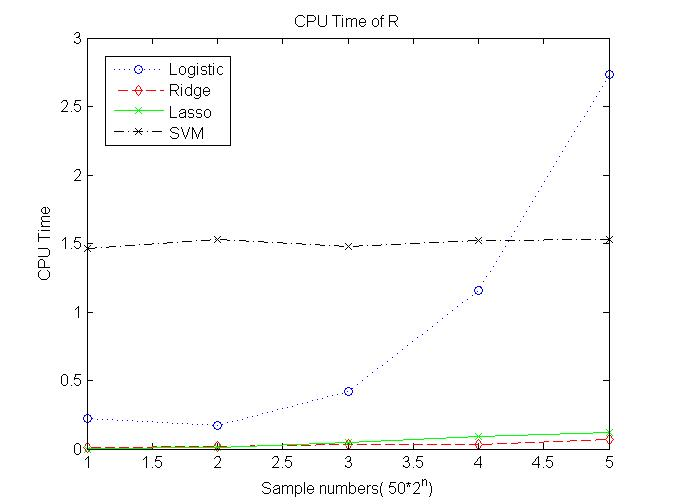
\includegraphics[width=0.8\textwidth, height=0.5\textheight]{cputime_r.jpg}

    \end{figure}

\end{block}

\column{2.3in}
\begin{block}{CPU Time for Python}
We changed the number of samples from 50 to 800, doubled each time to test the running time for the different machine learning methods:\\
\begin{figure}
     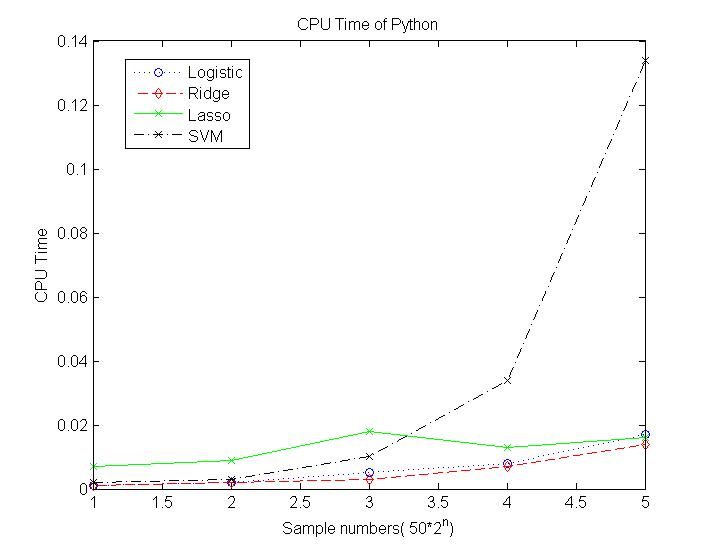
\includegraphics[width=0.8\textwidth, height=0.5\textheight]{cputime_python.jpg}

    \end{figure}
\end{block}

\end{columns}

\begin{block}{Results:}
Logistic and svm methods took long time than the other two in R , svm and lasso took long time in python.\\

\end{block}


\end{frame}

\begin{frame}
\frametitle{Numerical results}
\begin{block}{Comparison of CPU time for python and R }
\begin{center}
 \begin{figure}
     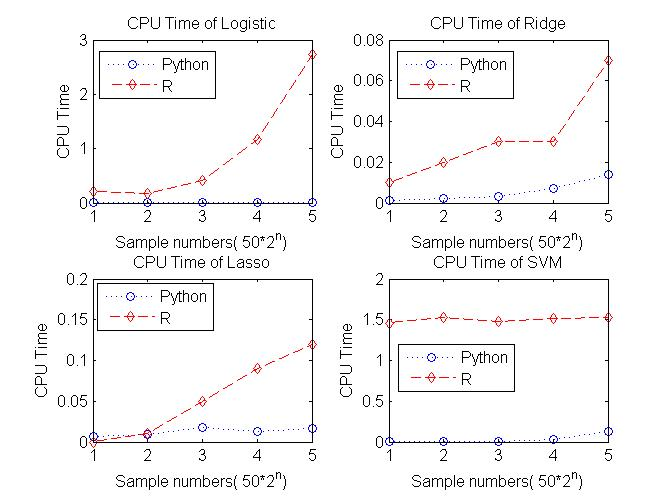
\includegraphics[width=0.8\textwidth, height=0.7\textheight]{cputime_python_r.jpg}

    \end{figure}
\end{center}
\end{block}

\begin{block}{Results:}
Python took smaller time for all the four methods compared with R.
\end{block}

\end{frame}

\begin{frame}
\frametitle{Numerical results:}

\begin{block}{Accuracy rate:}
\begin{table}[h!]\large
  \caption{Accuracy rate}
\begin{center}
    \begin{tabular}{| c | c| c | }
    \hline
    Methods& Python &  R\\
    \hline
Logistic  &69.8\%&	68.4\%\\
Ridge($\lambda$=1)&73.9\%	&77.4\%\\
Lasso($\lambda$=0.01)&78.6\%&	79.0\%\\
svm(linear)&72.4\%	&71.8\%\\
svm(poly)&74.3\%&	71.2\%\\
svm(rbf)&75.1\%	&72.8\%\\
\hline
\end{tabular}
\end{center}
\end{table}
\end{block}

\begin{block}{Results:}
\begin{itemize}
        \item lasso ($\lambda$=0.01) and svm (rbf) performed good for both two languages. 
        \item Python performed better in most cases but the difference is not significant.
    \end{itemize}

\end{block}
\end{frame}


\begin{frame}
\frametitle{Numerical results:}
\begin{block}{Predicted}
\begin{equation}
R_t^{GS} = \sum_{i=1:5}{\sum_{j=1:454}\beta_{i,j}R_{t-i}^j}
\end{equation}
\end{block}

\begin{block}{Predict:}
\begin{table}[h!]\large
  \caption{Accuracy rate and CPU time}
\begin{center}
    \begin{tabular}{| c | c|c|}
    \hline
    Methods& Accuracy rate& CPU time \\
    \hline
Logistic  &51.2\%&0.1210\\
Ridge($\lambda$=1)&54.0\%&0.1230\\
Lasso($\lambda$=0.01)&49.2\%&0.0940\\
svm(linear)&52.8\%&1.1931\\
svm(poly)&45.6\%&1.2800	\\
svm(rbf)&47.2\%&1.2921\\
Bayesian Glasso&51.6\%&around two hours\\
\hline
\end{tabular}
\end{center}
\end{table}
\end{block}
\end{frame}



\section{Future work}
\begin{frame}
\frametitle{Future work}
    \begin{itemize}
        \item  Compare with the time series model, such as Garch(machine learning methods can consider the whole economic environment while time series cannot)
        \item  Deal with the high frequency data instead of daily data
      \end{itemize}
\end{frame}

\section{Questions}
\begin{frame}
\frametitle{QA}
\begin{center}
\huge{Thanks a lot and Questions}
\end{center}
\end{frame}

\section{Section no.1} 
\frame{\frametitle{Title} 
Each frame should have a title.
}
\subsection{Subsection no.1.1  }
\frame{ 
Without title somethink is missing. 
}
%
\newcommand<>{\hover}[1] {\uncover#2 {
	\begin{tikzpicture}[remember picture,overlay,fill opacity=1]
    \draw [fill opacity=1] (current page.south west)
	rectangle (current page.north east);
	\node at (current page.center) {#1};
	\end{tikzpicture}}
	}

\begin{frame}
   \frametitle{A frame}
      Some text
      \hover<2>{
      \begin{minipage}{0.8\linewidth}
        \begin{block}{A block hovering above the slide}
        I am visible on slide two.
        \end{block}
      \end{minipage}
      }
\end{frame}
\section{Section no. 2} 
\subsection{Lists I}
\frame{\frametitle{unnumbered lists}
\begin{itemize}
\item Introduction to  \LaTeX  
\item Course 2 
\item Termpapers and presentations with \LaTeX 
\item Beamer class
\end{itemize} 
}

\frame{\frametitle{lists with pause}
\begin{itemize}
\item Introduction to  \LaTeX \pause 
\item Course 2 \pause 
\item Termpapers and presentations with \LaTeX \pause 
\item Beamer class
\end{itemize} 
}

\subsection{Lists II}
\frame{\frametitle{numbered lists}
\begin{enumerate}
\item Introduction to  \LaTeX  
\item Course 2 
\item Termpapers and presentations with \LaTeX 
\item Beamer class
\end{enumerate}
}
\frame{\frametitle{numbered lists with pause}
\begin{enumerate}
\item Introduction to  \LaTeX \pause 
\item Course 2 \pause 
\item Termpapers and presentations with \LaTeX \pause 
\item Beamer class
\end{enumerate}
}

\section{Section no.3} 
\subsection{Tables}
\frame{\frametitle{Tables}
\begin{tabular}{|c|c|c|}
\hline
\textbf{Date} & \textbf{Instructor} & \textbf{Title} \\
\hline
WS 04/05 & Sascha Frank & First steps with  \LaTeX  \\
\hline
SS 05 & Sascha Frank & \LaTeX \ Course serial \\
\hline
\end{tabular}}


\frame{\frametitle{Tables with pause}
\begin{tabular}{c c c}
A & B & C \\ 
\pause 
1 & 2 & 3 \\  
\pause 
A & B & C \\ 
\end{tabular} }


\section{Section no. 4}
\subsection{blocs}
\frame{\frametitle{blocs}

\begin{block}{title of the bloc}
bloc text
\end{block}

\begin{exampleblock}{title of the bloc}
bloc text
\end{exampleblock}


\begin{alertblock}{title of the bloc}
bloc text
\end{alertblock}
}
\end{document}

